\documentclass[a4paper,12pt]{ETHexercise}
\usepackage{bbm}

\input{preamble}

\usepackage{multirow}
\title{NLP Assignment}
\begin{document}
\setserie{1}


\newcommand{\pair}[2]{{\langle #1 , #2 \rangle}}
\newcommand{\score}[2]{\text{score}_{\theta}(\langle #1, #2 \rangle, \boldsymbol{w})}
\newcommand{\sscore}[1]{\text{score}_{\theta}(#1, \boldsymbol{w})}

\lectureheader{Prof. Ryan Cotterell}
{}
{\Large Natural Language Processing}{Fall 2022}
\begin{center}
	{\Huge Simon Wachter: Assignment 2}\\
	\quad\newline
	siwachte@ethz.ch, 19-920-198\\
	\quad\newline
	\timestamp
\end{center}

\begin{question}\\
	\begin{subquestion}
		Prove that the expectation semiring satisfies the semiring axioms:\\
		\begin{itemize}
			\item  $(\R \times \R, \oplus, \mathbf{0})$ must be a commutative monoid with identity element $\mathbf{0}$:
			      \begin{align}
				      \left(\pair{x}{y} \oplus \pair{x'}{y'}\right) \oplus \pair{x''}{y''} & =       \pair{x + x'}{y + y'}      \oplus \pair{x''}{y''}              \\
				                                                                           & = \pair{x + x' + x''}{y + y' + y''}                                    \\
				                                                                           & = \pair{x}{y} \oplus \pair{x' + x''}{y' + y''}                         \\
				                                                                           & = \pair{x}{y} \oplus \left(\pair{x'}{y'} \oplus \pair{x''}{y''}\right)
			      \end{align}
			      \begin{align}
				      \mathbf{0} + \pair{x}{y} & = \pair{0}{0} \oplus \pair{x}{y} \\
				                               & = \pair{0 + x}{0 + y}            \\
				                               & = \pair{x}{y}                    \\
				                               & = \pair{x + 0}{y + 0}            \\
				                               & = \pair{x}{y} + \mathbf{0}
			      \end{align}
			      \begin{align}
				      \pair{x}{y} + \pair{x'}{y'} & = \pair{x + x'}{y + y'}       \\
				                                  & = \pair{x' + x}{y' + y}       \\
				                                  & = \pair{x'}{y'} + \pair{x}{y}
			      \end{align}
			\item $(\R \times \R, \otimes, \mathbf{1})$ must be a monoid with identity element $\mathbf{1}$:
			      \begin{align}
				      \left(\pair{x}{y} \otimes \pair{x'}{y'} \right) \otimes \pair{x''}{y''} & = \pair{x \cdot x'}{x \cdot y' + y \cdot x'} \otimes \pair{x''}{y''}                              \\
				                                                                              & = \pair{x \cdot x' \cdot x''}{x \cdot x' \cdot y'' + (x \cdot y' + y \cdot x') \cdot x''}         \\
				                                                                              & = \pair{x \cdot x' \cdot x''}{x \cdot x' \cdot y'' + x \cdot y' \cdot x'' + y \cdot x' \cdot x''} \\
				                                                                              & = \pair{x}{y} \otimes \pair{x' \cdot x''}{x' \cdot y'' + y' \cdot x''}                            \\
				                                                                              & = \pair{x}{y} \otimes \left(\pair{x'}{y'} \otimes \pair{x''}{y''}\right)
			      \end{align}
			      \begin{align}
				      \mathbf{1} \otimes \pair{x}{y} & = \pair{1}{0} \otimes \pair{x}{y} \\
				                                     & = \pair{1 \cdot x}{1 \cdot y}     \\
				                                     & = \pair{x}{y}                     \\
				                                     & = \pair{x \cdot 1}{y \cdot 1}     \\
				                                     & = \pair{x}{y} \otimes \mathbf{1}
			      \end{align}
			\item Multiplication left and right distributes over addition:
			      \begin{align}
				      \pair{x}{y} \otimes \left(\pair{x'}{y'} \oplus \pair{x''}{y''}\right) & = \pair{x}{y} \otimes \pair{x' + x''}{y' + y''}                                                          \\
				                                                                            & = \pair{x \cdot x' + x \cdot x''}{x \cdot y' + x \cdot y'' + y \cdot x' + y \cdot x''}                   \\
				                                                                            & = \pair{x \cdot x'}{x \cdot y' + y \cdot x'} \oplus \pair{x \cdot x''}{x \cdot y'' + y \cdot x''}        \\
				                                                                            & = \left(\pair{x}{y} \otimes \pair{x'}{y'}\right) \oplus \left(\pair{x}{y} \otimes \pair{x''}{y''}\right)
			      \end{align}
			      \begin{align}
				      \left(\pair{x}{y} \oplus \pair{x'}{y'}\right) \otimes \pair{x''}{y''} & = \pair{x + x'}{y + y'} \otimes \pair{x''}{y''}                                                              \\
				                                                                            & = \pair{x \cdot x'' + x' \cdot x''}{x \cdot y'' + x' \cdot y'' + y \cdot x'' + y' \cdot x''}                 \\
				                                                                            & = \pair{x \cdot x''}{x \cdot y'' + y \cdot x''} \oplus \pair{x' \cdot x''}{x' \cdot y'' + y' \cdot x''}      \\
				                                                                            & = \left(\pair{x}{y} \otimes \pair{x''}{y''}\right) \oplus \left(\pair{x'}{y'} \otimes \pair{x''}{y''}\right)
			      \end{align}
			\item Multiplication by $\mathbf{0}$ annihilates $\R \times \R$:
			      \begin{align}
				      \mathbf{0} \otimes \pair{x}{y} & = \pair{0}{0} \otimes \pair{x}{y}       \\
				                                     & = \pair{0 \cdot x}{0 \cdot y}           \\
				                                     & = \pair{0}{0}                           \\    &= \mathbf{0}         \\
				                                     & = \pair{0}{0}                           \\
				                                     & = \pair{x \cdot 0}{y \cdot 0}           \\
				                                     & =       \pair{x}{y} \otimes \pair{0}{0} \\
				                                     & = \pair{x}{y} \otimes \mathbf{0}
			      \end{align}
		\end{itemize}
	\end{subquestion}
	\begin{subquestion}
		Our initial graph looks like \cref{figure:graph}.
		\begin{figure}[H]
			\centering
			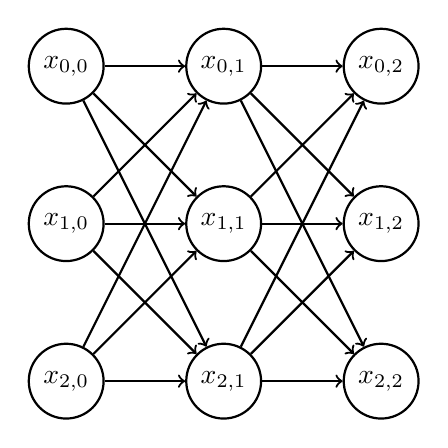
\begin{tikzpicture}[node distance={20mm}, thick, main/.style = {draw, circle}]
				\node[main] (0) {$x_{0,0}$};
				\node[main] (1) [below of=0]{$x_{1,0}$};
				\node[main] (2) [below of=1]{$x_{2,0}$};

				\node[main] (3) [right of=0]{$x_{0,1}$};
				\node[main] (4) [below of=3]{$x_{1,1}$};
				\node[main] (5) [below of=4]{$x_{2,1}$};

				\node[main] (6) [right of=3]{$x_{0,2}$};
				\node[main] (7) [below of=6]{$x_{1,2}$};
				\node[main] (8) [below of=7]{$x_{2,2}$};

				\draw[->] (0) -- (3);
				\draw[->] (0) -- (4);
				\draw[->] (0) -- (5);

				\draw[->] (1) -- (3);
				\draw[->] (1) -- (4);
				\draw[->] (1) -- (5);

				\draw[->] (2) -- (3);
				\draw[->] (2) -- (4);
				\draw[->] (2) -- (5);

				\draw[->] (3) -- (6);
				\draw[->] (3) -- (7);
				\draw[->] (3) -- (8);

				\draw[->] (4) -- (6);
				\draw[->] (4) -- (7);
				\draw[->] (4) -- (8);

				\draw[->] (5) -- (6);
				\draw[->] (5) -- (7);
				\draw[->] (5) -- (8);

			\end{tikzpicture}
			\caption[]{The initial graph}
			\label{figure:graph}
		\end{figure}
		Where the columns represent the words in $\mathbf{w}$ and the rows represent different tags.
		We use the algorithm from the script:\\
		\begin{algorithm}[H]
			\SetAlgoLined
			\caption{Forward pass}
			\label{algorithm:forward}
			$\beta(\mathbf{w}, t_0) = 1$\\
			\For{$n = 1 \to N$}{
				$\beta(\mathbf{w}, t_n) = \sum_{t_{n-1} \in \mathcal{T}} \exp(\score{\langle t_{n-1}}{t_n\rangle}) \otimes \beta(\mathbf{w}, t_{n-1})$
			}
		\end{algorithm}
		When we now lift the CRF into the expectation semiring, the forward propagation algorithm changes to:\\
		\begin{algorithm}[H]
			\SetAlgoLined
			\caption{Forward pass}
			\label{algorithm:forward_semi}
			$\beta(\mathbf{w}, t_0) = \langle 1, 0 \rangle$\\
			\For{$n = 1 \to N$}{
				$\beta(\mathbf{w}, t_n) = \oplus_{t_{n-1} \in \mathcal{T}} \langle w, -w \log w \rangle \otimes \beta(\mathbf{w}, t_{n-1})$
			}
		\end{algorithm}
		Where $w = \exp(\score{\langle t_n}{t_{n+1}\rangle})$.\\
		The output of the forward algorithm lifted into the semiring will yield:\\
		\begin{align}
			\bigoplus_{t_{1:N} \in T^{n}} \overset{N}{\bigotimes_{n=1}} \langle w, -w \log w \rangle
		\end{align}
		We want to show that the result of the forward propagation lifted in the semiring is the same as the unnormalized Entropy:
		\begin{align}
			H_u(T_{w}) & = -\sum_{\mathbf{t} \in \mathcal{T}^N} \exp(score_{\boldsymbol{\theta}} (\mathbf{t},\boldsymbol{w})) score_{\boldsymbol{\theta}} (\mathbf{t},\boldsymbol{w}) \label{eq:1b_to_show} \\
		\end{align}
		We show this by induction. Starting with the base case where $N = 1$:\\
		\begin{align}
			\bigoplus_{t_{1} \in T^{1}} \overset{1}{\bigotimes_{n=1}} \langle w, -w \log w \rangle & = \bigoplus_{t_{1} \in T^{1}} \langle \exp(\score{t_0}{t_1}),                     \\
			                                                                                       & \qquad -\exp(\score{t_0}{t_1}) \log(\exp(\score{t_0}{t_1})) \rangle               \\
			                                                                                       & = \bigoplus_{t \in T} \biggl< \exp(\sscore{t}),                         \nonumber \\
			                                                                                       & \qquad  -\exp(\sscore{t}) \log(\exp(\sscore{t})) \biggr>                          \\
			                                                                                       & = \biggl< \sum_{t \in T} \exp(\sscore{t}),                              \nonumber \\
			                                                                                       & \qquad -\sum_{t \in T} \exp(\sscore{t}) \log(\exp(\sscore{t})) \biggr>
		\end{align}
		Our induction hypothesis is the following:\\
		\begin{align}
			\bigoplus_{t_{1:i} \in T^{i}} \overset{i}{\bigotimes_{n=1}} \langle w, -w \log w \rangle = \left\langle \sum_{t \in T^{i}} \exp(\sscore{t}), -\sum_{t \in T^{i}} \exp(\sscore{t}) \log(\exp(\sscore{t})) \right\rangle
		\end{align}
		Meaning we assume that $\beta(\mathbf{w}, t_i)$ corresponds to the unnormalized entropy of all sequences of lenght $i$.\\
		Now we proceed with the induction step, where $i \rightarrow i + 1$:\\
		\begin{align}
			 & \bigoplus_{t_{1:i+1} \in T^{i+1}} \overset{i+1}{\bigotimes_{n=1}} \langle w, -w \log w \rangle \nonumber                                                                       \\ & = \bigoplus_{t_{1:i+1} \in T}  \left( \bigoplus_{t_{1:i} \in T^{i}} \overset{i}{\bigotimes_{n=1}} \langle w, -w \log w \rangle \right) \otimes \langle w, -w \log(w) \rangle \\
			 & \overset{\text{I.H.}}{=} \bigoplus_{t_{1:i+1} \in T} \left\langle \sum_{t \in T^{i}} \exp(\sscore{t}), -\sum_{t \in T^{i}} \exp(\sscore(t)) \sscore{t} \right\rangle \nonumber \\
			 & \otimes \left\langle \exp(\score{t_i}{t_{i+1}}), -\exp(\score{t_i}{t_{i+1}}) \score{t_i}{t_{i+1}}\right\rangle \label{eq:after_ih}
		\end{align}
		We will now analyze both parts of the semiring separately:
		\begin{align}
			 & \left(\sum_{t \in T^{i}} \exp(\sscore{t}) \right) \exp(\score{t_i}{t_{i+1}})                \\
			 & = \sum_{t \in T^{i}} \exp(\sscore{t}) + \score{t_i}{t_{i+1}}               \label{eq:semil}
		\end{align}
		And the second part:
		\begin{align}
			 & \left( \sum_{t \in T^{i}} \exp(\sscore{t}) \right) -\exp(\score{t_i}{t_{i+1}}) \score{t_i}{t_{i+1}} \nonumber                   \\
			 & \quad + \left( -\sum_{t \in T^{i}} \exp(\sscore(t)) \sscore{t} \right) \exp(\score{t_i}{t_{i+1}})                               \\
			 & = -\sum_{t \in T^{i}} \exp(\sscore{t} + \score{t_i}{t_{i+1}}) \score{t_i}{t_{i+1}} \nonumber                                    \\
			 & \quad -\left( \sum_{t \in T^{i}} \exp(\sscore(t)) \sscore{t} \right) \exp(\score{t_i}{t_{i+1}})                                 \\
			 & = -\sum_{t \in T^{i}} \exp(\sscore{t} + \score{t_i}{t_{i+1}}) \score{t_i}{t_{i+1}} \nonumber                                    \\
			 & \quad - \sum_{t \in T^{i}} \exp(\sscore{t} + \score{t_i}{t_{i+1}}) \sscore{t}                                                   \\
			 & = -\sum_{t \in T^{i}} \exp(\sscore{t} + \score{t_i}{t_{i+1}}) \left( \sscore{t} + \score{t_i}{t_{i+1}} \right) \label{eq:semir}
		\end{align}
		We can now combine the two parts to get with \cref{eq:after_ih}:
		\begin{align}
			 & \bigoplus_{t_{1:i+1} \in T} \left\langle \sum_{t \in T^{i}} \exp(\sscore{t}), -\sum_{t \in T^{i}} \exp(\sscore(t)) \sscore{t} \right\rangle \nonumber               \\
			 & \quad \otimes \left\langle \exp(\score{t_i}{t_{i+1}}), -\exp(\score{t_i}{t_{i+1}}) \score{t_i}{t_{i+1}}\right\rangle                                                \\
			 & \overset{\text{def. } \otimes}{=} \bigoplus_{t_{1:i+1} \in T} \biggl\langle \left(\sum_{t \in T^{i}} \exp(\sscore{t}) \right) \exp(\score{t_i}{t_{i+1}}), \nonumber \\
			 & \quad \left( \sum_{t \in T^{i}} \exp(\sscore{t}) \right) -\exp(\score{t_i}{t_{i+1}}) \score{t_i}{t_{i+1}} \nonumber                                                 \\
			 & \quad + \left( -\sum_{t \in T^{i}} \exp(\sscore(t)) \sscore{t} \right) \exp(\score{t_i}{t_{i+1}}) \biggr\rangle                                                     \\
			 & \overset{\cref{eq:semil}}{=} \bigoplus_{t_{1:i+1} \in T} \biggl\langle \sum_{t \in T^{i}} \exp(\sscore{t}) + \score{t_i}{t_{i+1}}, \nonumber                        \\
			 & \quad \left( \sum_{t \in T^{i}} \exp(\sscore{t}) \right) -\exp(\score{t_i}{t_{i+1}}) \score{t_i}{t_{i+1}} \nonumber                                                 \\
			 & \quad + \left( -\sum_{t \in T^{i}} \exp(\sscore(t)) \sscore{t} \right) \exp(\score{t_i}{t_{i+1}}) \biggr\rangle                                                     \\
			 & \overset{\cref{eq:semir}}{=} \bigoplus_{t_{1:i+1} \in T} \biggl\langle \sum_{t \in T^{i}} \exp(\sscore{t}) + \score{t_i}{t_{i+1}}, \nonumber                        \\
			 & \quad -\sum_{t \in T^{i}} \exp(\sscore{t} + \score{t_i}{t_{i+1}}) \left( \sscore{t} + \score{t_i}{t_{i+1}} \right) \biggr\rangle                                    \\
			 & \overset{\text{def. } \oplus}{=} \biggl\langle \sum_{t_{i+1} \in T} \sum_{t \in T^{i}} \exp(\sscore{t}) + \score{t_i}{t_{i+1}}, \nonumber                           \\
			 & \quad \sum_{t_{i+1} \in T} \sum_{t \in T^{i}} \exp(\sscore{t} + \score{t_i}{t_{i+1}}) \left( \sscore{t} + \score{t_i}{t_{i+1}} \right) \biggr\rangle                \\
			 & = \left\langle \sum_{t \in T^{i+1}} \exp(\sscore{t}), -\sum_{t \in T^{i+1}} \exp(\sscore{t}) \sscore{t} \right\rangle
		\end{align}
		Which concludes our induction proof and we have shown that \cref*{eq:1b_to_show} holds.
	\end{subquestion}
	\begin{subquestion}
		We want to prove:\\
		\begin{align}
			H(T_w) & = Z(\boldsymbol{w})^{-1} H_U(T) + \log(Z(\boldsymbol{w})
		\end{align}
		\begin{align}
			H(T_w) & = -\sum_{t \in T^{N}} p(t \:|\: w) \cdot \log(p(t \:|\: w))                                                                                                         &  & \text{(def. H)} \\
			       & = -\sum_{t \in T^{N}} \frac{\exp(\sscore{t})}{Z(\boldsymbol{w})} \log \left( \frac{\exp(\sscore{t})}{\sum_{t' \in T^N} \exp(\sscore{t'})} \right)                   &  & \text{(def. p)} \\
			       & = -\sum_{t \in T^{N}} \frac{\exp(\sscore{t})}{Z(\boldsymbol{w})} \log \left( \frac{\exp(\sscore{t})}{Z(\boldsymbol{w})} \right)                                                          \\
			       & = -\sum_{t \in T^{N}} \frac{\exp(\sscore{t})}{Z(\boldsymbol{w})} (\sscore{t} - \log Z(\boldsymbol{w}))                                                                                   \\
			       & = -\sum_{t \in T^{N}} \frac{\exp(\sscore{t}) \sscore{t} - \exp(\sscore{t}) \log Z(\boldsymbol{w}))}{Z(\boldsymbol{w})}                                                                   \\
			       & = -\sum_{t \in T^{N}} \frac{\exp(\sscore{t}) \sscore{t}}{Z(\boldsymbol{w})} + \sum_{t \in T^{N}} \frac{\exp(\sscore{t}) \log Z(\boldsymbol{w}))}{Z(\boldsymbol{w})}                      \\
			       & = H_U(T_{\boldsymbol{w}}) Z(\boldsymbol{w})^{-1}  + \frac{\log(Z(\boldsymbol{w}))}{Z(\boldsymbol{w})} \sum_{t \in T^{N}} \exp(\sscore{t})                                                \\
			       & = H_U(T_{\boldsymbol{w}}) Z(\boldsymbol{w})^{-1}  + \log(Z(\boldsymbol{w}))                                                                                                              \\
		\end{align}
	\end{subquestion}
	\begin{subquestion}
		We want to show that $H(T_w)$ can be computed in $\mathcal{O}(N \cdot |\mathcal{T}|^2)$.\\
		We do this by looking at the identity given in the previous subquestion and show that each term can be computed in at most $\mathcal{O}(N \cdot |\mathcal{T}|^2)$. As stated in the exercise $\log(Z(\boldmath{w}))$ can be computed in $\mathcal{O}(N \cdot |\mathcal{T}|^2)$. In exercise b) we have shown that with the expectation semiring we can calculate $H_U(T_w)$ with one forward/backward pass. \cref{algorithm:forward_semi} shows that the forward pass can be done in $\mathcal{O}(N \cdot |\mathcal{T}|)$, for the outer loop over the word length and for each iteration the sum over all possible taggings. The last term, $Z(\boldmath{w})$, can also be calculated in $\mathcal{O}(N \cdot |\mathcal{T}|)$, by running a forward/backwards pass without a semiring. This is shown in the lectures "Efficiently Computing the Normalizer", where we use  the distributive property of the product to calculate the normalizer with a linear number of terms. When we have all the subterms we only need a multiplication and an addition to arrive at $H(T_w)$.\\\\
		We can calculate the gradient by doing backpropagation over its computation graph. Hence, this can be done in the same bound as $\mathcal{O}(N \cdot |T|^2)$
	\end{subquestion}
\end{question}
\begin{question}\\
	\begin{subquestion}
		We again show the correctness by induction.\\

		\textbf{Base case ($|\boldmath{w}|=1$):}\\
		Our base case is a sequence with length $1$. After dequeueing the first element from the queue, which is the initialization element, we push elements for all possible taggings of the first word. In the next iteration, due to the priority queue structure we dequeue the element with the highest score. This is now a complete tagging for our sequence of length $1$ and it has the highest score.\\\\
		\textbf{Induction hypothesis}:\\
		The first sequence of length $i$ that is popped from the queue has the highest score among all sequences of length $i$.\\\\
		\textbf{Induction step ($i \rightarrow i+1$)}:\\
		Here we have two cases, one where the best tagging for sequence of length $i+1$ contains the best tagging for sequence of length $i$ as a prefix and one where it does not.\\
		\textbf{Case 1 ($t_{1:i} \in t_{1:i+1}$)}:\\
		Here $t_{1:i}$ denotes the a tagging for $w_1, \dots, w_i$.
		This case is straight forward, as per our induction hypothesis we know that $t_{1:i}$ is the best tagging for sequence of length $i$ and will therefore be the first element for sequence of length $i$ that is popped from the queue. The reasoning is the same as in the base case, all possible taggings of the next word are pushed to the queue and the element with the highest score is popped next.\\
		\textbf{Case 2 ($t_{1:i} \notin t_{1:i+1}$)}:\\
		Because our scores are in $\mathcal{R}_{\leq 0}$ we know that when we add to a sequence we can only decrease the score. Assume that the best tagging for length $i+1$ $T_{1:i+1}$ has score $s_{i+1}$. We then have two cases for all taggings $t_{1:k}$ where $k \leq i$. Either they are smaller or equal to $s_{i+1}$, then we do not care about them, since they cannot be used for the best tagging because we can only decrease them even more. Or they are larger than $s_{i+1}$, then we know that they will get popped before $T_{1:i+1}$, because they have a higher score. Therefore we know that the subtagging of $T_{1:i+1}$ $t'_{1:i}$ will be popped before any tagging with length $i+1$. This holds by contradiction, as otherwise $T_{1:i+1}$ would not be the best tagging.
	\end{subquestion}
	\begin{subquestion}
		We want to show that as Viterbi calculates the best tagging of lenght $i$ and ending with tag $t$ in $\gamma[i, t]$, so does Dijkstra.\\
		First we look at the dimension of $\gamma$, we know that for the Viterbi algorithm $\gamma$ has dimensions $\mathcal{R}^{N \otimes |\mathcal{T}|}$. We can clearly see that Dijkstra matches these dimensions, as for every possible tuple of tags $t \in \mathcal{T}$ and lenght $1 \leq i \leq N$ we have a score in $\gamma$. This holds because we save all pairs in an array and only allow distinct pairs in our queue (priority is updated when we have an overlap).\\
		To prove that the values are equivalent as well, we perform a contradiction proof:\\
		We assume that the score $s_{i}$ of tagging $T_{1:i}$ is not the best tagging of length $i$ and it's score is saved in $\gamma[i, t]$. Then there must exist a tagging $T_{1:i}'$ with score $s_{i}'$ that is better than $T_{1:i}$. Going back to the algorithm and our argument of exercise a) we know that all subtaggings $T_{1:k}'$ for $k \leq i$ have a higher score than $s_{i}'$ and therefore must have been popped from the queue before $\langle i, t \rangle$ and hence $\gamma[i, t]$ would be set to $s_{i}'$. This contradicts our assumption and therefore $s_{i}$ must be the best tagging of length $i$ and it's score is saved in $\gamma[i, t]$.
	\end{subquestion}
	\begin{subquestion}
		The normal Dijkstra with a priority queue based on a heap runs in $\mathcal{O}(|V| \log(|V|) + |E|)$. Our graph has $|\mathcal{T}| \cdot |\mathbf{w}|$ vertices as we have all possible taggins for each word. The edges are bound by $|\mathcal{T}|^2 \cdot |\mathbf{w}|$. This bound holds, becasuse each tag for a word has a connection to all other tags for the next word. When combining these insights we get the following runtime bound:
		\begin{align}
			\mathcal{O}(|\mathcal{T}||\mathbf{w}| \log(|\mathcal{T}||\mathbf{w}|) + |\mathcal{T}|^2 \cdot |\mathbf{w}|)
		\end{align}
		Viterbi:
		\begin{align}
			\mathcal{O}(|\mathbf{w}| \cdot |T|^2)
		\end{align}
	\end{subquestion}
	\begin{subquestion}
		The problem with the given semiring, is that multiple scores for a given tagging can affect the priority. This is a problem because we want the priority to be representative of the best score and not depend on other scores, which may be much worse. Hence, this semiring would not always have the best tagging of a given lenght $i$ popped first.
	\end{subquestion}
	\begin{subquestion}
		The property that we need from our semiring, are the ones that we use in our proof. One of which is $s_{1:i} \geq s_{1:i+1}$. Since we are using the $\otimes$ operator to build $s_{1:i+1}$ from $s_{1:i}$, this gives as constraints on the operator. Our priority queue must always return the tagging with the best score, hence we need the $\oplus$ to be a max operator. We could also have used a min operator, but then we would have to negate the scores.\\
	\end{subquestion}
\end{question}
\begin{question}\\
	Link to Colab Notebook: \url{https://colab.research.google.com/drive/1lFGpgB3MTTJZGb9akxGsRegdfDDEdf_p?usp=sharing}
	\\
	Question e):\\
	The naive viterbi implementation is clearly the slowest, which matches our expectation. Dijkstra is the second fastest, with a runtime of $34.8$ ms and backward viterbi is the fastest with $25.1$ ms (local runtimes, but matches results on colab). These observations match our expectations.
	I did the training for and g) outside of the notebook, just with a single python script as I was getting reduced performance and errors when running in the notebook.\\
	Output for g):\\
	\begin{verbatim}
		Starting training with beta 1.0
		Epoch 0, batch 0
		Epoch 0, batch 20
		...
		Epoch 0, batch 360
		Epoch 0, batch 380
		-------------------------
		Epoch: 1 / 3
		Development set accuracy: 0.8933365941047668
		-------------------------
		Epoch 1, batch 0
		Epoch 1, batch 20
		...
		Epoch 2, batch 360
		Epoch 1, batch 380
		-------------------------
		Epoch: 2 / 3
		Development set accuracy: 0.906506359577179
		-------------------------
		Epoch 2, batch 0
		Epoch 2, batch 20
		...
		Epoch 2, batch 360
		Epoch 2, batch 380
		-------------------------
		Epoch: 3 / 3
		Development set accuracy: 0.9176903367042542
		-------------------------
	\end{verbatim}
	\begin{verbatim}
		Starting training with beta 10.0
		Epoch 0, batch 0
		Epoch 0, batch 20
		...
		Epoch 0, batch 360
		Epoch 0, batch 380
		-------------------------
		Epoch: 1 / 3
		Development set accuracy: 0.8931728601455688
		-------------------------
		Epoch 1, batch 0
		Epoch 1, batch 20
		...
		Epoch 1, batch 360
		Epoch 1, batch 380
		-------------------------
		Epoch: 2 / 3
		Development set accuracy: 0.9124546051025391
		-------------------------
		Epoch 2, batch 0
		Epoch 2, batch 20
		...
		Epoch 2, batch 360
		Epoch 2, batch 380
		-------------------------
		Epoch: 3 / 3
		Development set accuracy: 0.9162563681602478
		-------------------------
	\end{verbatim}
	\begin{verbatim}
		Starting training with beta 0.1
		Epoch 0, batch 0
		Epoch 0, batch 20
		...
		Epoch 0, batch 360
		Epoch 0, batch 380
		-------------------------
		Epoch: 1 / 3
		Development set accuracy: 0.9024679660797119
		-------------------------
		Epoch 1, batch 0
		Epoch 1, batch 20
		...
		Epoch 1, batch 360
		Epoch 1, batch 380
		-------------------------
		Epoch: 2 / 3
		Development set accuracy: 0.9182560443878174
		-------------------------
		Epoch 2, batch 0
		Epoch 2, batch 20
		...
		Epoch 2, batch 360
		Epoch 2, batch 380
		-------------------------
		Epoch: 3 / 3
		Development set accuracy: 0.9221615791320801
		-------------------------
	\end{verbatim}
\end{question}
\end{document}

%%% Local Variables:
%%% mode: latex
%%% TeX-master: t
%%% End: